\documentclass[12pt,a4paper]{article}
\usepackage[a4paper,top=1.5cm, bottom=1.5cm, left=1.5cm, right=1.5cm]{geometry}
\usepackage[T2A]{fontenc}
\usepackage[utf8]{inputenc}
\usepackage[russian]{babel}
\usepackage{amsmath}
\usepackage{amssymb}
\usepackage{graphicx}
\usepackage{floatrow}
\usepackage{booktabs}
\usepackage{wrapfig}
\usepackage{lipsum}
\usepackage{subcaption}

\newcommand{\figref}[1]{(См. рис. \ref{#1})}
\newcommand{\e}[1]{\text{$\cdot10^{#1}$}}

\title{Лабораторная работа 2.4.1\\ Определение теплоты испарения жидкости}
\author{Симанкович Александр \\ Б01-104}
\date{09.03.2022}

\usepackage{float}
\restylefloat{table}

\begin{document}
	\maketitle
	
	\section*{Цель работы}
	
	Измерение давления насыщенного пара жидкости при разной температуре. \\
	Вычисление по полученным данным теплоты испарения с помощью уравнения Клапейрона–Клаузиуса.
	
	\section*{Оборудование и приборы} 
	Термостат; герметический сосуд, заполненный исследуемой жидкостью; отсчетный микроскоп.
	
	
	\section*{Теоретическое введение}
	
	Испарением называется переход вещества из жидкого в газообразное состояние. Оно происходит на свободной поверхности жидкости. При испарении с поверхности вылетают молекулы, образуя над ней пар. Для выхода из жидкости молекулы должны преодолеть силы молекулярного сцепления. Кроме того, при испарении совершается работа против внешнего давления $ P $, поскольку объем жидкости меньше объема пара. Не все молекулы жидкости способны совершить эту работу, а только те из них, которые обладают достаточной кинетической энергией. Поэтому переход части молекул в пар приводит к обеднению жидкости быстрыми молекулами, т.е. к ее охлаждению. Чтобы испарение проходило без изменения температуры, к жидкости нужно подводить тепло. Количество теплоты, необходимое для изотермического испарения одного моля жидкости при внешнем давлении, равном упругости ее насыщенных паров, называется молярной теплотой испарения (парообразования).
	
	Теплоту парообразования жидкостей можно измерить непосредственно при помощи калориметра. Такой метод, однако, не позволяет получить точных результатов из-за неконтролируемых потерь тепла, которые трудно сделать малыми. В настоящей работе для определения теплоты испарения применен косвенный метод, основанный на формуле Клапейрона–Клаузиуса:
	
	\begin{equation}\label{Kl-Kl}
		\frac{dP}{dT}=\frac{L}{T\left(V_2-V_1\right)}.
	\end{equation}
	
	Здесь $ P $ -- давление насыщенного пара жидкости при температуре $ T $, $ T $ -- абсолютная температура жидкости и пара, $ L $ -- теплота испарения жидкости, $ V_2 $ -- объем пара, $ V_1 $ -- объем жидкости. Найдя из опыта $ dP/dT $, $ T $, $ V_2 $ и $ V_1 $, можно определить $ L $ путем расчета. Величины $ L $, $ V_2 $ и $ V_1 $ в формуле \eqref{Kl-Kl} должны относиться к одному и тому же количеству вещества; мы будем относить их к одному молю.
	
	В нашем приборе измерения производятся при давлениях ниже атмосферного. В этом случае задача существенно упрощается.
	
	При нашей точности опытов величиной $ V_1 $ в \eqref{Kl-Kl} можно пренебречь.
	
	Обратимся теперь к $ V_2 $, которое в дальнейшем будем обозначать просто $ V $. Объем $ V $ связан с давлением и температурой уравнением Ван-дер-Ваальса:
	
	\begin{equation}\label{VDV}
		\left(P+\frac{a}{V^2}\right)\left(V-b\right)=RT.
	\end{equation}
	
	Из табличных данных следует, что $ b $ одного порядка с $ V_1 $. В уравнении Ван-дер-Ваальса величиной $ b $ следует пренебречь. Пренебрежение членом $ a/V^2 $ по сравнению с $ P $ вносит ошибку менее 3\%. При давлении ниже атмосферного ошибки становятся еще меньше. Таким образом, при давлениях ниже атмосферного уравнение Ван-дер-Ваальса для насыщенного пара мало отличается от уравнения Клапейрона. Положим поэтому
	
	\begin{equation}\label{Volume}
		V=\frac{RT}{P}.
	\end{equation}
	
	Подставляя \eqref{Volume} в \eqref{Kl-Kl}, пренебрегая $ V_1 $ и разрешая уравнение относительно $ L $, найдем
	
	\begin{equation}\label{final}
		L=\frac{RT^2}{P}\frac{dP}{dT}=-R\frac{d(\ln P)}{d(1/T)}.
	\end{equation}
	
	В нашем опыте температура жидкости измеряется термометром, давление пара определяется при помощи манометра, а производные $ dP/dT $ или $ d(\ln P)/d(1/T) $ находятся графически как угловой коэффициент касательной к кривой $ P(T) $ или соответственно к кривой, у которой по оси абсцисс отложено $ 1/T $, а по оси ординат $ \ln P $.
	
	
	\section*{Экспериментальная установка}
	
	На рисунке изображена схема установки.  Наполненный водой резервуар 1 играет роль термостата. Нагревание термостата производится спиралью 2, подогреваемой электрическим током. Для охлаждения воды в термостате через змеевик 3 пропускается водопроводная вода. Вода в термостате перемешивается воздухом, поступающим через трубку 4. Температура воды измеряется термометром 5.В термостат погружен прибор 6 с исследуемой жидкостью.Над ней находится насыщенный пар. (перед заполнением прибора воздух из него был откачан). Давление насыщенного пара определяется по ртутному манометру соединенному с исследуемым объемом. Отсчет показаний манометра производится при помощи микроскопа.\\
	
	\begin{figure}[h]
		\begin{center}
			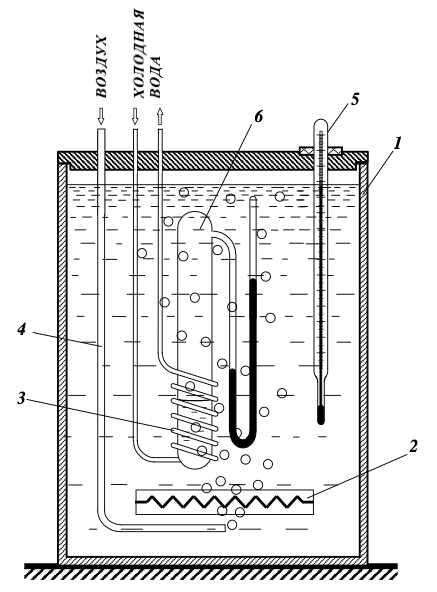
\includegraphics[width=0.3\linewidth]{scheme1.jpg}
		\end{center}
		\caption{Схема установки}
		\label{img2}
	\end{figure}	
	
	
	\section*{Ход работы}
	
	Данные эксперимента для процесса при повышении и понижении температуры занесены в таблицу.
	
	Систематические погрешности измерений: $$ \sigma_T = 0.2 K \;\;\; \sigma_h = \sqrt{6} \cdot 0.1 \; \text{мм}\;\;\; \varepsilon_h \approx 1 \%$$
	
	\begin{table}[H]
%		\centering
		\input{heating.tex}
		\hspace{0.1\textwidth}
		\input{freezing.tex}
		
		\caption{Данные при нагреве и охлаждении}		
	\end{table}

	Нули в последних ячейках столбцов $\frac{dp}{dT}$ возникли из-за того, что количество точек производной на одну меньше, чем количество измерений. В расчетах эти нули не используются.

	Воспользуемся двумя вариантами линеаризации.
	
	$$\frac{dP}{dT} = \frac{L}{R} \cdot \frac{P}{T^2}$$
	$$\ln{P} = -\frac{L}{R} \cdot \frac{1}{T} + C$$
	
	Перейдем к расчету зависимостей. Обработку проведем методом наименьших квадратов:
	
	$$y = Ax + B,$$
	
	где $$A = \frac{r_{xy}}{ \sigma_x^2},$$
	$$B = \overline{y} - A\overline{x}.$$
	
	\begin{table}
	\begin{tabular}{rrrrrrrrr}
	\hline
		$\overline{x}$ & $\sigma_x^2$ & $\overline{y}$ & $\sigma_y^2$ & $r_{xy}$ & $a$ & $\Delta a$ & $b$ & $\Delta b$ \\
		3.30e-03 & 3.18e-09 & 9.22 & 8.01e-02 & -1.59e-05 & -5017.70 & 38.63 & 25.76 & 0.13 \\
	\hline
	\end{tabular}
	\begin{tabular}{rrrrrrrrr}
	\hline
		$\overline{x}$ & $\sigma_x^2$ & $\overline{y}$ & $\sigma_y^2$ & $r_{xy}$ & $a$ & $\Delta a$ & $b$ & $\Delta b$ \\
		3.35e-03 & 5.63e-09 & 9.04 & 1.19e-01 & -2.58e-05 & -4584.45 & 56.75 & 24.37 & 0.19 \\
	\end{tabular}
	\caption{$\ln p (\frac{1}{T})$ \\ Нагревание (верхние) и охлаждение (нижние) коэффициенты}
	\end{table}

	\begin{table}
	\begin{tabular}{rrrrrrrrr}
	\hline
		$\overline{x}$ & $\sigma_x^2$ & $\overline{y}$ & $\sigma_y^2$ & $r_{xy}$ & $a$ & $\Delta a$ & $b$ & $\Delta b$ \\
		1.10e-01 & 6.61e-04 & 560.00 & 3.27e+04 & 3.99e+00 & 6033.97 & 934.11 & -102.80 & 105.38 \\
	\end{tabular}
	\begin{tabular}{rrrrrrrrr}
	\hline
		$\overline{x}$ & $\sigma_x^2$ & $\overline{y}$ & $\sigma_y^2$ & $r_{xy}$ & $a$ & $\Delta a$ & $b$ & $\Delta b$ \\
		9.55e-02 & 7.45e-04 & 463.02 & 6.03e+04 & 4.77e+00 & 6402.78 & 1413.03 & -148.24 & 140.30 \\
	\hline
	\end{tabular}
	\caption{$\frac{dp}{dT} (\frac{p}{T^2})$ \\ Нагревание (верхние) и охлаждение (нижние) коэффициенты}
	\end{table}

\newpage
	Для оценки погрешностей используем следующие формулы:
	$$\Delta A =  2 \sqrt{\frac{1}{n-2} \left( \frac{\sigma_y^2}{\sigma_x^2} - A^2 \right)},$$
	$$\Delta B = \Delta A \sqrt{\sigma_x^2 + \overline{x}^2},$$

	\begin{figure}[H]
		\includegraphics{pic1.pdf}
		\caption{Зависимость давления насыщенных паров от температуры}
	\end{figure}

	\begin{figure}[H]
		\includegraphics{pic2.pdf}
		\caption{Линеаризация $\ln p (\frac{1}{T})$)}
	\end{figure}
	
	\begin{figure}[H]
		\includegraphics{pic3.pdf}
		\caption{Линеаризация $\frac{dp}{dT} (\frac{p}{T^2})$}
	\end{figure}
	
\section*{Вывод}

	Как видно из итоговой таблицы и графиков, на оценку результатов работы сильно влияет выбранный метод линеаризации. Второй способ дает на порядок большую случайную погрешность. 
	
	В таблице также учтена погрешность эксперимента (см. Теоретическое введение)
	
	\begin{table}[H]
		\caption{Вывод}
		\label{tab:itog}
		\centering
		\footnotesize
		\begin{tabular}{l|r|r}
			\toprule
			$ $ & Нагрев, $\frac{\text{Дж}}{\text{кг}}$& Охлаждение, $\frac{\text{Дж}}{\text{кг}}$ \\ \midrule
			Линеаризация $\ln{p}(\frac{1}{T})$          & $(9.1 \pm 0.3)\e{5}$ & $(8.3 \pm 0.3)\e{5}$  \\ \midrule 
			Линеаризация $\frac{dP}{dT}(\frac{P}{T^2})$ & $(10.9 \pm 1.8)\e{5}$ & $(12 \pm 3)\e{5} $  \\ \midrule
			Табличная величина 							& $9.07\e{5} $ & $9.07\e{5} $  \\ 
			\bottomrule
		\end{tabular}
	\end{table}

	Учесть реальные погрешности первого способа является сложной задачей. Метод наименьших квадратов позволяет оценить только случайную погрешность, тогда как в опыте явно присутствует систематическая погрешность. Дополнительной проблемой оказался процесс охлаждения. Он происходил быстрее, чем нагрев, вследствие чего квазистатичность процесса нарушалась. Вероятно по этой причине первый коэффициент является весьма точным, тогда как второй имеет большое отклонение.
	
\end{document}